\documentclass[../../main.tex]{subfiles}
\begin{document}

{\bf [解]}
(1) $t\to 0$の時を考えるので，$t$が十分$O$に近いとして $|\cos2x|=\cos2x$と考えて良い．
この時平均値の定理から，
\begin{align}
  F(t)=\dfrac{\displaystyle \int_0^{\frac{\pi t}{2}}\cos2x\,dx}{t}=\dfrac{\pi}{2}\cos2p \quad \left(0<p<\dfrac{\pi t}{2}\right)
\end{align}
をみたす$p$がある．はさみうちの定理より$t\to 0$の時$p\to 0$で $\cos2x$は連続だから，求める極限値は
\begin{align}
 \lim_{t\to 0} F(t) = \dfrac{\pi}{2}\cos(2\lim_{t\to 0} p )=\dfrac{\pi}{2} \cos(2\cdot 0) = \dfrac{\pi}{2}
\end{align}
である．

(2)
被積分関数の絶対値を外すと
\begin{align}
\begin{split}
F(t)&=
  \begin{cases}\displaystyle
  \dfrac{1}{t}\displaystyle\int_0^{\frac{\pi}{2}t}\cos2x\,dx & \left(0<t\le\dfrac{1}{2}\right) \\[2mm]
  \dfrac{1}{t}\left\{\displaystyle\int_0^{\frac{\pi}{4}}\cos2x\,dx-\int_{\frac{\pi}{4}}^{\frac{\pi}{2}t}\cos2x\,dx\right\} & \left(\dfrac{1}{2}\le t\le1\right)
  \end{cases} \\
&=
  \begin{cases}\displaystyle
  \dfrac{1}{2t}\sin\pi t & \left(0<t\le\dfrac{1}{2}\right) \\[2mm]
  \dfrac{1}{2t}(2-\sin\pi t) & \left(\dfrac{1}{2}\le t\le1\right)
  \end{cases}
\end{split}
\end{align}
となる．
前者は$(0,0)$と$\left(t,\dfrac{1}{2}\sin\pi t\right)$を結ぶ直線の傾き，後者は$(0,0)$と$\left(t,1-\dfrac{1}{2}\sin\pi t\right)$を結ぶ直線の傾きを表す．
これらのグラフは，端点での傾きにも注意して以下のようになる．

\begin{figure}[htb]
\centering
% ===== 図1: 0 < t <= 1/2 の幾何学的イメージ =====
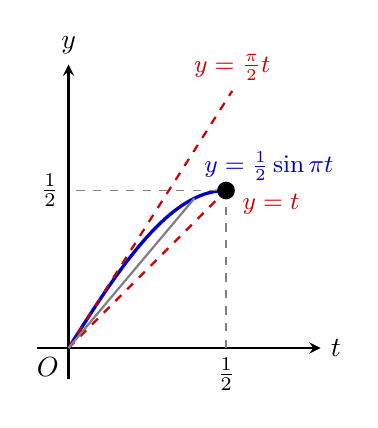
\begin{tikzpicture}[scale=4, >=stealth]
  % 座標軸
  \draw[->, thick] (-0.1, 0) -- (0.8, 0) node[right] {$t$};
  \draw[->, thick] (0, -0.1) -- (0, 0.9) node[above] {$y$};
  \node[below left] at (0,0) {$\text{O}$};

  % y = (1/2)sin(\pi t) の曲線 (0 <= t <= 1/2)
  \draw[domain=0:0.5, smooth, very thick, blue!80!black] plot (\x, {0.5*sin(180*\x)});
  \node[blue!80!black, font=\small, above right] at (0.4, 0.5) {$y = \frac{1}{2}\sin\pi t$};

  % 接線 y = (\pi/2)t （t=0 での接線）
  \draw[dashed, red!80!black, thick, domain=0:0.52] plot (\x, {1.5708*\x}) node[above, font=\small] {$y = \frac{\pi}{2}t$};

  % 接線 y = t （t=1/2 での線）
  \draw[dashed, red!80!black, thick, domain=0:0.52] plot (\x, \x) node[below right, font=\small] {$y = t$};


  % 任意の点 (t, y) を通る割線 (原点からの直線)
  \draw[gray, thick] (0,0) -- (0.4, 0.4755);

  % ガイド線とプロット点
  \draw[dashed, gray] (0.5, 0) -- (0.5, 0.5) -- (0, 0.5);
  \fill[black] (0.5, 0.5) circle (0.8pt);

  % 軸ラベル
  \node[below] at (0.5, 0) {$\frac{1}{2}$};
  \node[left] at (0, 0.5) {$\frac{1}{2}$};
\end{tikzpicture}
\hspace{1cm} % 左右の図の間隔
% ===== 図2: 1/2 <= t <= 1 の幾何学的イメージ =====
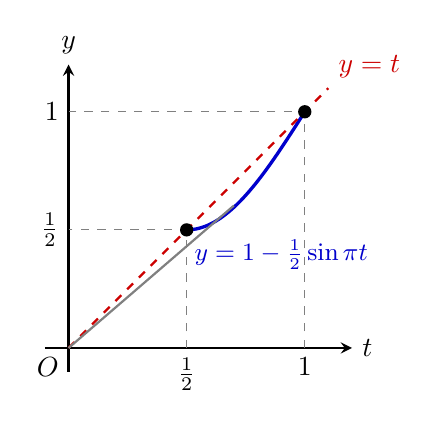
\begin{tikzpicture}[scale=3, >=stealth]
  % 座標軸
  \draw[->, thick] (-0.1, 0) -- (1.2, 0) node[right] {$t$};
  \draw[->, thick] (0, -0.1) -- (0, 1.2) node[above] {$y$};
  \node[below left] at (0,0) {$\text{O}$};

  % y = 1 - (1/2)sin(\pi t) の曲線 (1/2 <= t <= 1)
  \draw[domain=0.5:1, smooth, very thick, blue!80!black] plot (\x, {1 - 0.5*sin(180*\x)});
  \node[blue!80!black, font=\small, below] at (0.9, 0.5) {$y = 1 - \frac{1}{2}\sin\pi t$};

  % 直線 y = x （原点と (1,1) を結ぶ直線）
  \draw[dashed, red!80!black, thick, domain=0:1.1] plot (\x, {\x}) node[above right] {$y = t$};

  % 任意の点を通る割線 (原点からの直線)
  \draw[gray, thick] (0,0) -- (0.7, 0.603);

  % ガイド線とプロット点
  \draw[dashed, gray] (0.5, 0) -- (0.5, 0.5) -- (0, 0.5);
  \draw[dashed, gray] (1.0, 0) -- (1.0, 1.0) -- (0, 1.0);
  
  \fill[black] (0.5, 0.5) circle (0.8pt);
  \fill[black] (1.0, 1.0) circle (0.8pt);

  % 軸ラベル
  \node[below] at (0.5, 0) {$\frac{1}{2}$};
  \node[below] at (1.0, 0) {$1$};
  \node[left] at (0, 0.5) {$\frac{1}{2}$};
  \node[left] at (0, 1.0) {$1$};
\end{tikzpicture}
\caption{傾きとしての $F(t)$ の幾何学的意味}
\end{figure}

従って $y=F(t)$ のグラフの概形は下図のようになる．

\begin{figure}[htb]
\centering
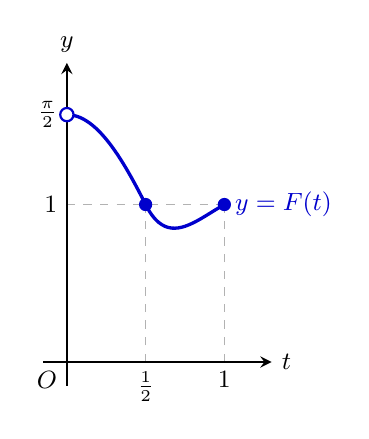
\begin{tikzpicture}[
  scale=2.0, 
  >=stealth, 
  every node/.style={font=\small} % ラベルサイズを統一して見やすく
]
  % 1. ガイド線（点線）と軸の目盛り補助
  \draw[dashed, gray!60] (0, 1.0) -- (1.0, 1.0);
  \draw[dashed, gray!60] (0.5, 0) -- (0.5, 1.0);
  \draw[dashed, gray!60] (1.0, 0) -- (1.0, 1.0);
  \draw[dashed, gray!60] (0, 1.571) -- (0.02, 1.571);

  % 2. 座標軸
  \draw[->, thick] (-0.15, 0) -- (1.3, 0) node[right] {$t$};
  \draw[->, thick] (0, -0.15) -- (0, 1.9) node[above] {$y$};
  \node[below left] at (0,0) {$\text{O}$};

  % 軸上の数値ラベル
  \node[left] at (0, 1.0) {$1$};
  \node[left] at (0, 1.571) {$\frac{\pi}{2}$};
  \node[below] at (0.5, 0) {$\frac{1}{2}$};
  \node[below] at (1.0, 0) {$1$};

  % 3. y = F(t) の曲線描画
  % 0 < t <= 1/2 : (1/2t)sin(pi t)
  \draw[domain=0.025:0.5, smooth, very thick, blue!80!black] 
    plot (\x, {sin(180*\x)/(2*\x)});
  
  % 1/2 <= t <= 1 : (1/2t)(2 - sin(pi t))
  \draw[domain=0.5:1.0, smooth, very thick, blue!80!black] 
    plot (\x, {(2 - sin(180*\x))/(2*\x)}) node[right, font=\small] {$y = F(t)$};

  % 4. 特徴的なプロット点
  % t -> 0 での除外点 (白抜き)
  \fill[white] (0, 1.571) circle (1.2pt);
  \draw[thick, blue!80!black] (0, 1.571) circle (1.2pt);

  % t = 1/2, 1 での定義点 (黒塗り)
  \fill[blue!80!black] (0.5, 1.0) circle (1.2pt);
  \fill[blue!80!black] (1.0, 1.0) circle (1.2pt);

\end{tikzpicture}
\caption{$y=F(t)$ のグラフの概形}
\end{figure}

したがって，$F(t)\ge1$となる$t$の範囲は，
\begin{align}
  0<t\le\dfrac{1}{2},\quad t=1
\end{align}
である．

\bigskip
\noindent\textbf{[解2]}
(2)
新しく
\begin{align}
 g(t)=\displaystyle\int_0^{\frac{\pi}{2}t}|\cos2x|dx
\end{align}
とおくと，$F(t)$は$(0,0)$と$(t,g(t))$の傾きである．
$y=g(t)$のグラフは，$\left(\dfrac{1}{2},g\left(\dfrac{1}{2}\right)\right)$を軸に対称である．$0<t\le\dfrac{1}{2}$の時，
\begin{align}
 g(t)=\dfrac{1}{2}\sin\pi t
\end{align}
だから$y=g(t)$のグラフは下のようになる．

\begin{figure}[htb]
\centering
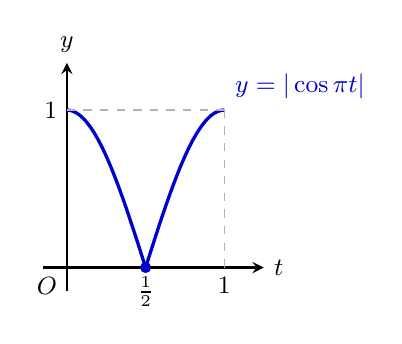
\begin{tikzpicture}[
  scale=2.0, 
  >=stealth, 
  every node/.style={font=\small}
]
  % 座標軸
  \draw[->, thick] (-0.15, 0) -- (1.25, 0) node[right] {$t$};
  \draw[->, thick] (0, -0.15) -- (0, 1.3) node[above] {$y$};
  \node[below left] at (0,0) {$\text{O}$};

  % y = |cos(\pi t)| の曲線
  \draw[domain=0:0.5, smooth, very thick, blue!80!black] plot (\x, {cos(180*\x)});
  \draw[domain=0.5:1.0, smooth, very thick, blue!80!black] plot (\x, {-cos(180*\x)}) 
    node[above right, font=\small] {$y = |\cos\pi t|$};

  % ガイド線と特徴点
  \draw[dashed, gray!60] (0, 1.0) -- (1.0, 1.0);
  \draw[dashed, gray!60] (0.5, 0) -- (0.5, 0);
  \draw[dashed, gray!60] (1.0, 0) -- (1.0, 1.0);

  % 軸ラベル
  \node[left] at (0, 1.0) {$1$};
  \node[below] at (0.5, 0) {$\frac{1}{2}$};
  \node[below] at (1.0, 0) {$1$};

  % 折り返し点 (t = 1/2) のプロット
  \fill[blue!80!black] (0.5, 0) circle (1.0pt);

\end{tikzpicture}
\caption{$y = |\cos\pi t|$ のグラフ}
\end{figure}


\begin{figure}[htb]
\centering
\begin{tikzpicture}[
  scale=2.0, 
  >=stealth, 
  every node/.style={font=\small}
]
  % 座標軸
  \draw[->, thick] (-0.15, 0) -- (1.25, 0) node[right] {$t$};
  \draw[->, thick] (0, -0.15) -- (0, 1.3) node[above] {$y$};
  \node[below left] at (0,0) {$\text{O}$};

  % y = g(t) の曲線
  % 0 <= t <= 1/2 : (1/2)sin(\pi t)
  \draw[domain=0:0.5, smooth, very thick, blue!80!black] plot (\x, {0.5*sin(180*\x)});
  % 1/2 <= t <= 1 : 1 - (1/2)sin(\pi t)
  \draw[domain=0.5:1.0, smooth, very thick, blue!80!black] plot (\x, {1 - 0.5*sin(180*\x)})
    node[right, font=\small] {$y = g(t)$};

  % ガイド線
  \draw[dashed, gray!60] (0, 0.5) -- (0.5, 0.5) -- (0.5, 0);
  \draw[dashed, gray!60] (0, 1.0) -- (1.0, 1.0) -- (1.0, 0);

  % 軸上の目盛り
  \node[left] at (0, 0.5) {$\frac{1}{2}$};
  \node[left] at (0, 1.0) {$1$};
  \node[below] at (0.5, 0) {$\frac{1}{2}$};
  \node[below] at (1.0, 0) {$1$};

  % 変曲点 (1/2, 1/2) と 端点 (1, 1)
  \fill[blue!80!black] (0.5, 0.5) circle (1.0pt);
  \fill[blue!80!black] (1.0, 1.0) circle (1.0pt);

  % 凹凸の指示矢印とラベル (手書き図に対応)
  \draw[<-, >=stealth, thin, gray!80!black] (0.22, 0.33) -- (0.15, 0.55) node[above, font=\footnotesize, black] {上に凸};
  \draw[<-, >=stealth, thin, gray!80!black] (0.78, 0.67) -- (0.85, 0.45) node[below, font=\footnotesize, black] {下に凸};

\end{tikzpicture}
\caption{$y = g(t)$ のグラフと凹凸}
\end{figure}

従って求める$t$の範囲は
\begin{align}
0<t\le\dfrac{1}{2} \ \text{または}\ t=1
\end{align}
である．

\end{document}
